\newpage
\section{Architettura generale}

L'applicativo \progetto\ è strutturato in un lato front-end ed un lato back-end, come mostrato dal diagramma seguente:

\begin{figure}[H]
	\centering
	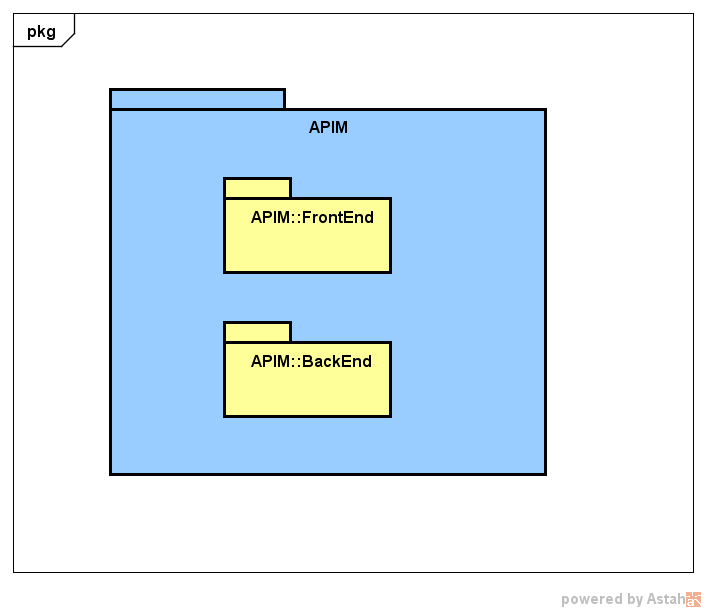
\includegraphics
	[width=0.7\linewidth]
	{UML/DiagrammiPackage/APIM.png}
	\caption{Package APIM}
\end{figure}

\newpage
\subsection{Front-end}
Nella parte front-end sono presenti i package \textit{node\_modules} e \textit{App}, che derivano dall'architettura dei componenti e framework scelti (AngularJS).

\begin{figure}[H]
	\centering
	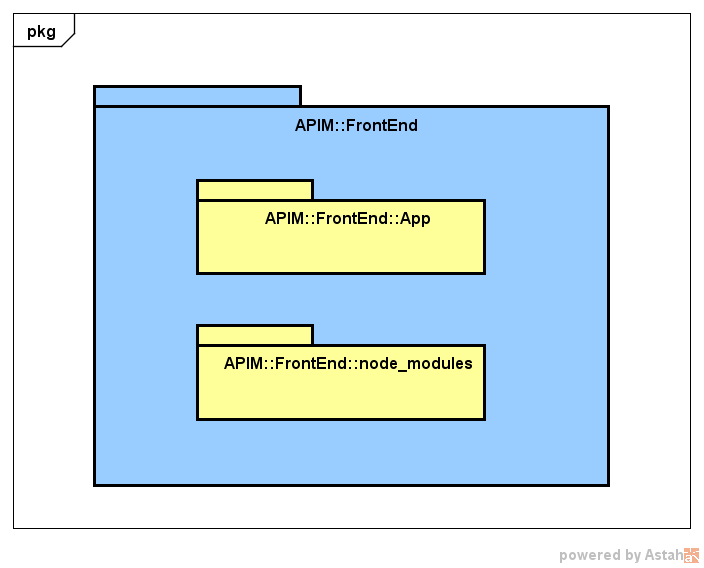
\includegraphics
	[width=0.7\linewidth]
	{UML/DiagrammiPackage/FrontEnd.png}
	\caption{Package APIM::FrontEnd}
\end{figure}

\begin{itemize}
	\item \textbf{Padre}: APIM;
	
	\item \textbf{Descrizione}: package contenente le componenti del front-end dell'applicazione;
	
	\item \textbf{Package contenuti}:
	\begin{itemize}
		\item \textbf{\textit{node\_modules}}: package contenente i riferimenti alle librerie esterne di JavaScript;
		
		\item \textbf{\textit{App}}: package contenente le componenti principali dell'applicazione.
	\end{itemize}
\end{itemize}

\newpage
\subsection{Back-end}
Nella parte back-end sono presenti i package \textit{Gateway} e \textit{Services} strutturati secondo un'architettura a microservizi, i quali hanno una dipendenza verso l'interfaccia \textit{ServiceInteractionHandler}.

\begin{figure}[H]
	\centering
	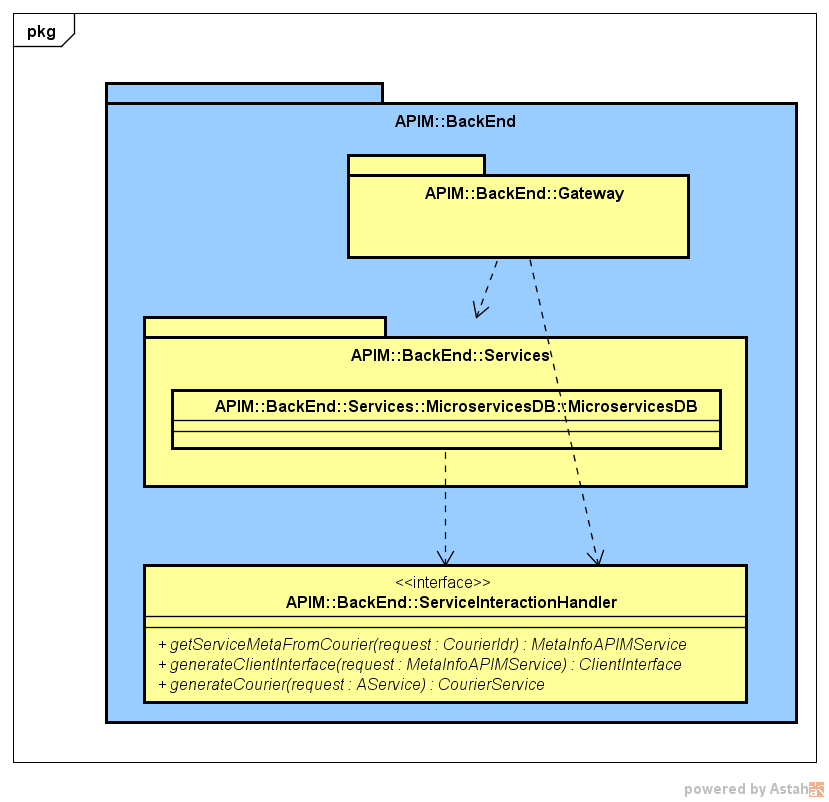
\includegraphics
	[width=0.7\linewidth]
	{UML/DiagrammiPackage/BackEnd.png}
	\caption{Package APIM::BackEnd}
\end{figure}

\begin{itemize}
	\item \textbf{Padre}: APIM;
	
	\item \textbf{Descrizione}: package contenente le componenti del back-end dell'applicazione;
	
	\item \textbf{Package contenuti}:
	\begin{itemize}
		\item \textbf{\textit{Gateway}}: package contenente le classi e le interfacce per il funzionamento dell'API Gateway;
		
		\item \textbf{\textit{Services}}: package contenente tutti i microservizi per le comunicazioni con i database.
	\end{itemize}
	\item \textbf{Classi contenute}:
	\begin{itemize}
		\item \textbf{\textit{ServiceInteractionHandler}}: interfaccia per la gestione delle comunicazioni dell'API Gateway e dei \textit{services}.
	\end{itemize}
\end{itemize}

Nelle sezioni verranno presentati i packages in maniera dettagliata.